\chapter{Architecture}
Within this chapter the architecture of the implemented software will be described in detail according to the used project structure of the visual studio solution.
	\section{Overview}
	
\begin{center}
	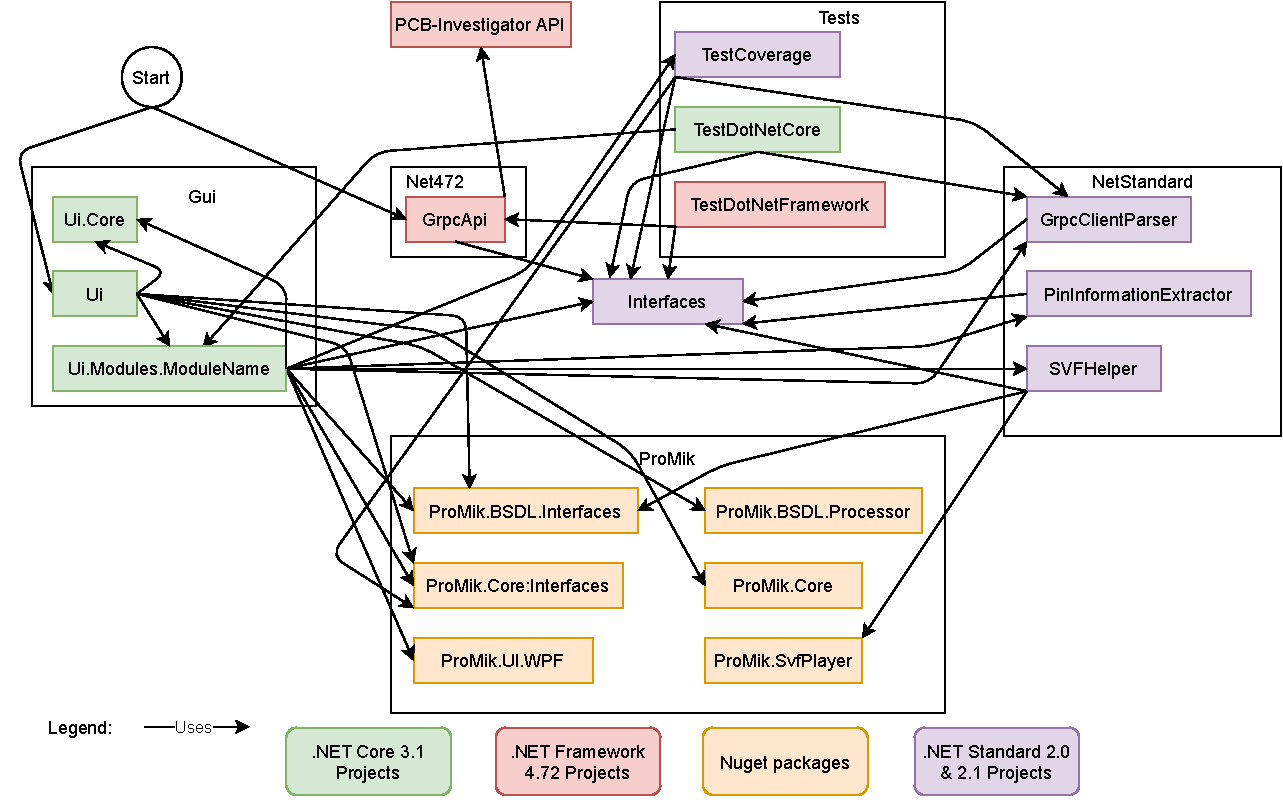
\includegraphics[width=1.00\textwidth]{figures/project structure.pdf}
	\begin{figure}[!h]
	\caption{Project overview}
	\label{fig:projectOverview}
	\end{figure}
\end{center}

As shown in \ref{fig:projectOverview} it will be clear that the whole project is organized in different kind of folders which contain C\# projects. On one side there is the \textbf{Gui} folder containing the following projects:
\begin{itemize}
	\item Ui.Core - This project contains the region names and the view model bases which should be inherited and was provided by the PRISM framework.
	\item Ui - Within the project the mainView and mainViewModel could be found (Was initially created by the PRISM framework)
	\item Ui.Modules.ModuleName - This project was basically created by the PRISM framework and contains all necessary events, interfaces, models, viewmodels and views for operating with all other referenced projects
\end{itemize}
On the other side there is the \textbf{Net472} folder with the project GrpcApi which contains the standalone software for referencing the \ac{PCB}-Investigator API and runs as a \ac{GRPC} server. Next the \textbf{NetStandard} folder contains the following projects:
\begin{itemize}
	\item GrpcClientParser - The \ac{GRPC} client project for communicating with the GrpcApi project for getting all parsed objects by the \ac{PCB}-Investigator API
	\item PinInformationExtractor - This project is being used for creation of textfiles in \ac{JSON} format containing all pin information of all \ac{JTAG} devices of one project.
	\item SVFHelper - This project is needed for creation of \ac{SVF} files in dependency on \ac{BSDL} files which should be referenced for \ac{JTAG} devices. Further it could play \ac{SVF} files with a programmer from ProMik which is connected to a boundary scan compatible \ac{JTAG} device
\end{itemize}
The \textbf{Tests} folder consists of the following projects:
\begin{itemize}
	\item TestCoverage - This project contains all boundary scan test according logic to be performed
	\item TestDotNetCore - Here there can be found different unit tests for the parser logic of the GrpcClientParser project
	\item TestDotNetFramework - This project contains unit tests to be performed using the GrpcApi project
\end{itemize}
Finally there were different \textbf{ProMik} related projects included by the nuget package manager of visual studio:
\begin{itemize}
	\item ProMik.BSDL.Interfaces - Contains all interfaces regarding the BSDL handling
	\item ProMik.BSDL-Processor - Contains the implementations regarding the BSDL processor
	\item ProMik.Core.Interfaces - The interfaces of core logic
	\item ProMik.Core - The implementations of core logic
	\item ProMik.UI.WPF - Contains different Ui elements which could be included (settings panel, logPanel \ac{etc.})
	\item ProMik.SvfPlayer - Contains the logic for creation and playing of \ac{SVF} files
\end{itemize}

	\section{Interfaces}
The Interfaces project was created as a .NET standart 2.0 project to make sure it could be referenced by any other projects which needs it. It has the following content:
\begin{itemize}
	\item Gui - Within this folder are just interfaces located which are related to the Gui logic
	\begin{itemize}
		\item IDialogSelector - It could be used for the handling of dialogs which should be shown either for file opening, saving or folder opening or saving
		\item ILogger - The system wide used interface for logging purposes which additionally will be written into a local logfile
	\end{itemize}
	\item Helper - A folder wich contains objects which were necessary for the two unit test related projects
	\begin{itemize}
		\item PcbTestObject - This is a helper class for unit test purposes
		\item PinTestObject - It is a helper class which is been included in the PcbTestObjects class and provides more detailed pin information
	\end{itemize}
	\item PcbInvestigator - That folder contains all \ac{PCB}-Investigator related interfaces and their implementations of the received objects
	\begin{itemize}
		\item IFunctionalAttributes - The interface which contains all functional related attributes
		\item IGeometricAttributes - A interface which contains all geometric and position related information
		\item INetComponent - This is the interface for representing a net object
		\item IPinComponent - That is a interface for describing a pin object
		\item IPCBComponent - An interface which contains all information about a PCBComponent
		\item Enums - Within that folder are the enumerations placed which were used within the IPCBComponent and IPinComponent for defining the componentType and pinType
		\item Implementations - In that folder are all implementations of the predefined interfaces of the PCBInvestigator objects located
	\end{itemize}
\end{itemize}

	\section{Grpc Server for using the PCB Investigator API}
This project is responsible for using the \ac{PCB}-Investigator API which is being created using the .NET Framework and was created as a console application using the .NET Framework 4.72 as well. It further derives a service which was provided by a \ac{GRPC} auto code generation as a server. The proto file itself which was used for the code generation contains three functions:
\begin{itemize}
	\item GetConvertedObjects(Request) returns (Result) - Within this function all objects of a specific project could be determined using the location to the project
	\item GetConvertedObjectsByZip(RequestZip) returns (Result) - That method obtains all objects by using the received project as zip file in bytes
	\item ClientAvailable(Empty) returns (StatusResult) - This function is being used to detect whether the client has a valid connection to the server using the settings or not
\end{itemize}

	\section{Grpc Client for connecting to the Server and parsing all objects}

	\section{GUI}

		\subsection{Events}

		\subsection{Helper}

		\subsection{Interfaces}

		\subsection{Implementations}

		\subsection{Model}

		\subsection{ViewModels}

		\subsection{Views}

		\subsection{MainView and MainViewModel}

	\section{Test coverage determination of loaded project}

	\section{Pin information extraction}

	\section{SVF file generator}

	\section{Unit tests}